%!TEX root = ../dokumentation.tex

\chapter{Theoretische Grundlagen}\label{cha:Grundlagen}
Für das bessere Verständnis des Themas soll dieses Kapitel die relevanten, theoretischen Grundlagen vermitteln,  und an das Kernthema heranführen. Dabei wird zunächst geklärt, worum es sich bei der Überwachung von IT-Infrastrukturen handelt, und soll Antworten auf Fragen wie "`Warum werden diese überwacht?"', "`Welche Komponenten sind zu unterscheiden?"' und "`Welche Technologien werden eingesetzt?"' geben. Danach soll der Begriff Logfiles genauer definiert werden, bevor die Funktionalität von MapReduce und Hadoop erläutert wird.

%TODO: Einleitung überarbeiten
<Einleitung in das Kapitel noch nicht wirklich rund. Überarbeiten!>

%Kurze Einleitung in das Kapitel. Beschreiben warum die Grundlagen notwendig sind. Auch darüber schreiben, dass nicht ALLE Grundlagen sondern lediglich die für das Verständnis der Arbeit notwendigen erklärt werden.

\section{Überwachung von IT-Infrastrukturen}\label{sec:UeberwachungIT}
Ziel der Überwachung ist es, durch Extraktion von Informationen und überprüfen von Komponenten, Aussagen über den Zustand einer oder mehrerer Komponenten innerhalb einer IT-Infrastruktur zu erhalten. Die durch die Überwachung erhobenen Basis-Informationen werden zur Optimierung der Performance und Verfügbarkeit eines Dienstes eingesetzt.

Nach Salm gibt es drei Arten von Komponenten die es zu unterscheiden gilt:

\begin{itemize}
	\item Netzwerk, um eine ausreichende Bandbreite und bestehende Übertragung zu sichern
	\item Ressourcen, um eine effiziente Lastverteilung innerhalb der Infrastruktur zu gewährleisten
	\item Anwendung, um Anwender schnellen, unkomplizierten Zugriff zu ermöglichen
\end{itemize}

Überwachungssysteme zeigen Administratoren die Up- und Downtime, sowie die Auslastung, von Soft- und Hardware an.\footcite[Vgl.][S. 8]{Salm.2007}

Um Aussagen über den Zustand einer Komponente treffen zu können, analysiert das Überwachungssystem eine Vielzahl von Informationen. Dabei werden unterschiedliche Techniken eingesetzt von einfachen Standard-Unix-Kommandozeilen-Tools bis hin zu intelligenten Agenten.

Diese Agenten werden auf der Zielkomponente installiert und sind als Hintergrundanwendung dauerhaft aktiv um immer die aktuellsten Informationen an das Überwachungssystem zu übermitteln.

Um eine hohe Qualität der Daten zu gewährleisten, werden die Agenten, entweder direkt oder über eine externe Schnittstelle, so konfiguriert, dass sie nur die Informationen ermitteln und übertragen, welche für das Überwachungssystem relevant sind. Agenten können auch eine direktere Rolle bei der Überwachung von Komponenten übernehmen, indem sie, anstatt oder zusätzlich zu den Informationen, die Daten selbst interpretieren, um Meldungen an das Überwachungssystem zu übermitteln.

In beiden fällen kombinieren Agenten selbst ermittelte Informationen mit bereits vorhandenen. Zu den selbst ermittelten Daten gehören unter anderem CPU und RAM Auslastung oder offene Ports. Bereits vorhandene Informationen können durch auf der Komponente laufende Software, oder durch die Komponente selbst, erzeugt werden.

Speziell Webseiten und deren Infrastrukturen, ist die Überwachung ein signifikanter Punkt bei der Qualitätssicherung. Die Verfügbarkeit eines Systems ist oft Teil von Dienstleistungsverträgen. Aus diesem Grund setzen IT-Dienstleister auf Monitoring Systeme wie \gls{Nagios} oder \gls{Zabbix}, um Informationen über die von ihnen administrierten Systeme zu erhalten. Auf allen zu überwachenden Systemen werden die entsprechenden Agenten installiert und aktiviert. Danach kann das Hauptsystem über die Agenten alle benötigten Informationen beziehen.

Von besonderem Interesse sind hier Logfiles. Aus ihnen lassen sich viele Informationen über den Zustand eines Systems ausgelesen. Dabei handelt es sich sowohl um Real- oder Near-Time, als auch historische Informationen.

%TODO: Überleitung zu Logfiles schreiben aus fokusieren auf web und monitoring systemen
%<Kurze Fokusierung auf Online Service. Welche Informationen werden hier im speziellen benötigt. Erwähnen von Monitoring Systemen. Funktion von Agenten, im zusammenspiel mit Monitoring Systemen, bei der analyse von Logfiles beschreiben und daraus die Überleitung zu Logfiles ableiten>

%Worum geht es bei der Überwachung? Was ist das Ziel? Warum braucht man eine Überwachung? Wie sieht diese i.d.R. Aus? Welche Kernpunkte gibt es in der Überwachung? \\
%Hier sollte die Überleitung zum nächsten Kapitel kommen d.h. Logfiles werden als letztes behandelt in diesem Kapitel, damit der Übergang sauber ist.

\section{Bedeutung von Logfiles}\label{sec:BedeutungVonLogfiles}
Nach Baur und Blasius bezeichnen Logfiles (oder auch Protokolldateien) \flqq [...] automatisch erstellte Dateien [..], in denen bestimmte Ereignisse elektronisch aufgezeichnet werden.\frqq\footcite[S. 847]{Baur.2014} Dabei werden sowohl negative wie auch positive Ereignisse protokolliert.

Bei Web-Servern, welche mit Apache \acs{HTTP} Server (später Apache) unter Linux betrieben werden, stellen syslog von Linux, sowie Error- und Access-Log von Apache, die Grundlage zur Überwachung des Servers. Sie lassen sich sehr einfach durch die in \autoref{sec:UeberwachungIT} beschriebenen Agenten überwachen, da sie einem klar vorgegebenen Standard folgen.

Im syslog von Linux werden alle Ereignisse protokolliert, welche im direkten Zusammenhang mit dem System stehen. Die Einträge folgen dabei der im \ac{RFC} 5424\footcite[RFC 5424,][]{RFC5424.2009} festgehaltenen Beschreibung (Da es sich bei RFC um keine offizielle Norm handelt, handelt es sich lediglich um eine Beschreibung, nicht um einen Standard).

Das Apache-Error-Log enthält diagnostische Informationen und protokolliert alle Fehler, welche bei der Verarbeitung einer Anfrage auftreten. \autoref{lst:BeispieleintragApacheErrorLog} zeigt, wie ein Eintrag in einem Error-Log aussehen könnte. Es lässt sich klar erkennen, wann der Fehler aufgetreten ist, was fehlgeschlagen ist und welches Modul betroffen ist. Ebenfalls sichtbar ist die \ac{IP}-Adresse des Clients, bei dem der Fehler aufgetreten ist. Die Einträge des Error-Logs entsprechen keiner Norm oder \ac{RFC} Beschreibung. Sie können nach der Installation individuell angepasst werden.\footcite[Vgl.][]{ApacheErrorLog.2015} \\

\begin{lstlisting}[caption=Beispieleintrag für ein Apache-Error-Log,label=lst:BeispieleintragApacheErrorLog]
[Fri Jun 12 10:42:29.902022 2015] ERROR [pid 35708:tid 4328636416] [client 192.168.172.15] File does not exist: /usr/local/apache2/htdocs/favicon.ico
\end{lstlisting}

Im Apache-Access-Log werden alle Anfragen an den Server protokolliert. Dabei wird gespeichert von welcher \ac{IP}-Adresse die Anfrage kam, wann die Anfrage gestartet wurde, welcher Art die Anfrage war und welcher Pfad angefragt wurde, sowie welcher Statuscode zurückgegeben wurde und wie groß die Antwort des Servers war (siehe \autoref{lst:BeispieleintragApacheAccessLog}). \\

\begin{lstlisting}[caption=Beispieleintrag für ein Apache-Access-Log,label=lst:BeispieleintragApacheAccessLog]
192.168.172.15 - Max [11/Jun/2015:13:55:36 -0700] "GET /dummy.gif HTTP/1.0" 200 2326
\end{lstlisting}

Wie beim Error-Log können die Einträge angepasst werden und folgen somit keiner Norm oder \ac{RFC}. Die Beispiele zeigen ebenfalls, wie unterschiedlich die Einträge für zwei Logfiles des gleichen Systems sein können.\footcite[Vgl.][]{ApacheAccessLog.2015}

Da es sich bei \ac{IP}-Adressen potenziell um Personenbezogenen Daten handelt, ist diese nach §3 Abs. 1 \ac{BDSG} geschützt\footcite[§3 Abs. 1 BDSG,][]{BDSG3.1990} (Potenziell Personenbezogen, da nicht ersichtlich ist, ob eine \ac{IP}-Adresse statisch oder dynamisch ist). Die Speicherung der \ac{IP}-Adresse ist daher nur gestattet, wenn der Anwender zustimmt, oder ein Grund für die Speicherung vorliegt, welcher §15 \ac{TMG} genügt.\footcite[§15 TMG,][]{TMG15.2007} Ist dies nicht der Fall, darf die \ac{IP} nicht Teil des Protokolleintrags sein. Die Standardeinstellung muss entsprechend verändert werden.

Da es sich bei dem im Zuge dieser Arbeit entwickelten Programm um eine prototypische Anwendung handelt, können die Datenschutzrichtlinien vorerst vernachlässigt werden. Es geht primär um die Anwendung eines Modells auf einen konkreten Fall.

Wie gezeigt wurde, gibt es keinen einheitlichen Standard für die Notation innerhalb von Logfiles. Dieser Umstand hat zur Folge, dass nur die üblichen Logfiles wie Error- oder Access-Log, über Agenten ausgewertet werden können, solange deren Notation nicht verändert wurde. Um dennoch Informationen über den Zustand eines Systems oder einzelner Module automatisiert zu erhalten, müssen entsprechende Anwendungen geschrieben werden. Da es sich hierbei um eine sehr große Menge an textbasierten Daten handelt, eignet sich hierfür besonders das MapReduce-Modell.

%<Zusammenfassung am ende des Kapitels. Aufzeigen das Logfiles unterschiedliche Notation besitzen und keinem einheitlichen Standard folgen. Erwähnen das die üblichen Logs trotz allem durch Agenten auswertbar sind, die Logs um die es später geht jedoch nicht. Aus dieser Aussage die verwendung von MapReduce begründen und daraus die Überleitung zu MapReduce bilden>

%Was sind Logfiles im allgemeinen? Was ist die Funktion eines Logfiles? Gibt es Standards? Wenn ja welche und wie sehen die aus? Werden die Standards im weiteren Verlauf der Arbeit noch einmal relevant sein (Ja/Nein begründen und erläutern)?

\section{Einführung in MapReduce}\label{sec:EinführungInMapReduce}
Die Google Mitarbeiter Jeffrey Dean und Sanjar Ghemawat veröffentlichten 2004 eine Arbeit, in welcher sie einen neuen Ansatz zur Verarbeitung von großen, unstrukturierten Daten beschrieben. Das in der Arbeit beschriebene Modell wurde als \textit{Map-Reduce} bezeichnet. Dabei wurde nicht nur beschrieben, wie man große Datenmengen durchsucht, auswertet und in Schlüssel-Wert-Paaren zusammenfasst. Die Clusterung von Jobs auf \gls{Commodity-Hardware} waren ebenfalls ein Bestandteil der Arbeit. Freiknecht schreibt weiter, dass diese Arbeit als Ursprung des Algorithmus bezeichnet wird, und somit Implementierungen wie Hadoop, Disco oder BashReduce inspiriert hat.\footcite[Vgl.][S. 42]{Freiknecht.2014}

Ein MapReduce Programm lässt sich i.d.R. in drei Bereiche unterteilen. Der Map-Phase, in welcher die Schlüssel-Wert-Paare aus den Eingabedaten erzeugt werden, der Combine-Phase, zur Aggregation der Paare, sowie der Reduce-Phase, in welcher die Daten ausgedünnt werden, bis nur noch ein Wert pro Schlüssel vorhanden ist (siehe \autoref{fig:DreiPhasenMapReduce}).

\begin{figure}[h]
	\centering
	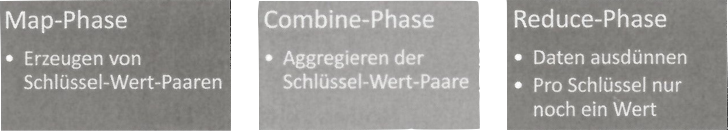
\includegraphics[width=.8\textwidth]{MapReduce_001.png}
	\caption{Die drei Phasen eines Map-Reduce-Prozesses\footnotemark}
	\label{fig:DreiPhasenMapReduce}
\end{figure}
\footnotetext{\cite[S. 42.]{Freiknecht.2014}}

Die Stärke von MapReduce, liegt in der Kombination von sequentieller und paralleler Verarbeitung. Die einzelnen Phasen von MapReduce werden sequentiell ausgeführt. Die Combine- oder Reduce-Phase kann nicht beginnen, bevor die Map-Phase abgeschlossen ist. Innerhalb der Phasen können die Aufgaben jedoch auf mehrere Instanzen verteilt und parallel verarbeitet werden. Diese Form der Verarbeitung entspricht dem Master-Worker-Modell.\footcite[Vgl.][S.1 f]{Karloff.2010}

Speziell bei der Parallelisierung von Tasks, welche wenig bis keine Abhängigkeit voneinander aufweise, stellt dieses Modell ein ideales Hilfsmittel dar. Die zentralen Elemente des Schemas bildet ein Master und $n$ Worker. Der Master startet die Verarbeitung, indem er ein gegebenes Problem aufarbeitet und eine Sammlung von Tasks erzeugt.  Die Tasks werden vom Master an die ihm bekannten Worker verteilt (Worker werden entweder vom Master selbst erzeugt oder melden sich bei diesem an). Die Worker arbeiten parallel und senden einen Statuscode an den Master, sobald der Task vollständig bearbeitet wurde (oder der Worker in einen Fehler läuft).\footcite[Vgl.][S. 80 ff]{Fey.2008} \autoref{fig:MasterWorkerInMR} zeigt die Anwendung des Master-Worker-Modells auf ein MapReduce Programm.

\begin{figure}[h]
	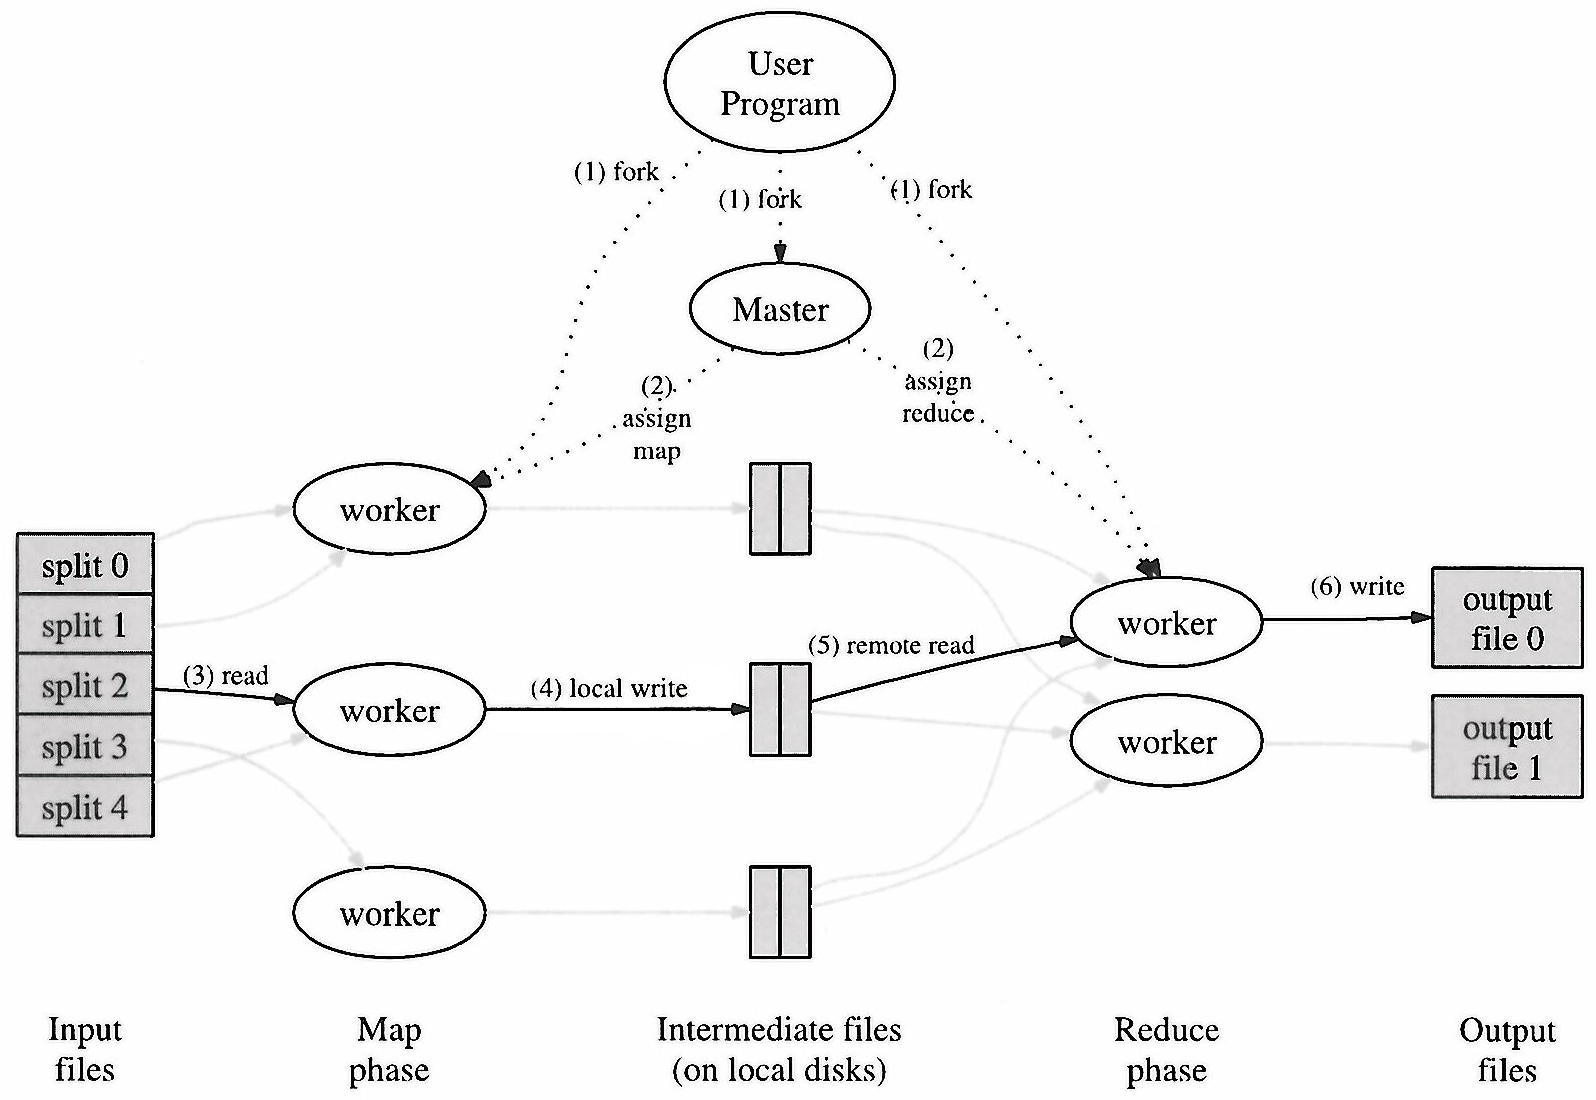
\includegraphics[width=1\textwidth]{MasterWorkerMR.png}
	\caption{Master-Worker in MapReduce\footnotemark}
	\label{fig:MasterWorkerInMR}
\end{figure}
\footnotetext{\cite[S. 3.]{Dean.2004}}

Im folgenden wird MapReduce zunächst formal definiert. Die Grundlage der Definition bildet das durch Karloff, Suri und Vassilvitskii beschriebene \ac{MRC} Model.\footcite[S. 3 f]{Karloff.2010} Danach soll die Funktionsweise anhand eines Beispiels weiter verdeutlicht werden.

\subsection{Formale Beschreibung von MapReduce}\label{subsec:FormaleBeschreibung}
Da es sich bei MapReduce um ein Modell zur Verarbeitung von Daten handelt, und nicht um einen Algorithmus, wird die durch Karloff et al. beschriebene \ac{MRC} verwendet, um eine Grundlage für die formale Definition zu haben. Dabei werden die drei Karakteristiken Funktion, Ausführungszeit und Speicherauslastung beschrieben.

Im Zentrum der Datenverarbeitung mit MapReduce steht das Schlüssel-Wert-Paar, welches als ein String Tupel $\langle k; v \rangle$, mit dem Schlüssel $k$ und dem dazu gehörenden Wert $v$. Die Eingabe für eine \ac{MRC} Maschine ist eine Liste von Schlüssel-Wert-Paaren $\langle k_i, v_i \rangle_{i=1}^{\mathbb{N}}$ mit einer Gesamtgröße im Speicher von $\sum_{i=1}^{\mathbb{N}}|k_i|+|v_i|$.

Die Map Funktion verarbeitet einen Tupel $\langle k; v \rangle$ zu einer Liste von neuen Schlüssel-Wert-Paaren $\langle k_1; v_1 \rangle, \langle k_2; v_2 \rangle, \dots, \langle k_n; v_n \rangle$.

Die Reduce Funktion erhält als Eingabeparameter einen Schlüssel $k$ sowie eine Sequenz von Werten $v_1, v_2, \dots, v_n$. Aus diesen erzeugt die Funktion eine Liste von Schlüssel-Wert-Paaren $\langle k; v_{k,1} \rangle, \langle k; v_{k,2} \rangle, \dots, \langle k; v_{k,n} \rangle$. Die Schlüssel der Tupel in der erzeugten Liste ist identisch mit dem Schlüssel, welcher an die Reduce Funktion übergeben wurde.

Aus diesen beiden Definitionen folgt, dass die Map Funktion Schlüssel nach belieben manipulieren kann. Für Reduce sind die Schlüssel jedoch unveränderlich.

Die Ausführung von MapReduce lässt sich wie folgt definieren. Sei $M$ die Menge aller Map und Reduce Funktionen $\langle \mu_1, \rho_1, \mu_2, \rho_2, \dots, \mu_R, \rho_R \rangle$ und $U_0$ eine Liste von Tupeln $\langle k; v \rangle$, dann gilt für die Ausführung von $M$ auf die Daten $U_0$:

Für $r = 1, 2, \dots, R$:

\begin{enumerate}
	\item \textbf{MAP:} $\forall \langle k; v \rangle \in U_{r-1}$ führe $\mu_r \in M$ mit $\langle k; v \rangle$ aus. Die Funktion erzeugt eine Liste neuer Tupel $\langle k_1; v_1 \rangle, \langle k_2; v_2 \rangle, \dots, \langle k_n; v_n \rangle$. Sei $U_r^{\prime}$ die Ausgabe für eine Eingabe $\langle k; v \rangle$, dann gilt: $U_r^{\prime} = \bigcup_{\langle k; v \rangle \in U_{r-1}} \mu_r(\langle k; v\rangle)$.
	\item \textbf{COMBINE:} $\forall k$ erzeuge Liste $V_{k,r}$ mit den Werten $v_i$, so dass gilt $\langle k; v_i \rangle \in U_r^{\prime}$.
	\item \textbf{REDUCE:} $\forall k$, übergebe $k$ und eine willkürliche Permutation von $V_{k,r}$ in eine Instanz von Reducer $\rho_r \in M$ zur Ausführung. Dieser erzeugt eine Liste von Tupeln $\langle k; v_1^{\prime} \rangle, \langle k; v_2^{\prime} \rangle, \dots, \langle k; v_n^{\prime} \rangle$. Sei $U_r$ die Ausgabe für die Eingabe $\langle k; V_{k,r} \rangle$, \\ dann gilt: $U_r = \bigcup_k \rho(\langle k; V_{k,r}\rangle)$.
\end{enumerate}

Die Verarbeitung wird beendet, wenn der letzte Reducer $\rho_R$ beendet wird. In der Definition wird die Möglichkeit zur Parallelisierung, der sequentiell ausgeführten Funktionen Map und Reduce deutlich. Sowohl Mapper als auch Reducer verarbeiten immer nur einen Tupel zeitgleich. Es können also mehrere Instanzen von $\mu_r$ und $\rho_r$ gestartet werden.\footcite[Vgl.][S. 2 f]{Karloff.2010}

Die Ausführungszeit von MapReduce kann nicht spezifiziert werden ohne ein Wissen über den Inhalt der Funktionen. Die Effizient hängt von den in den Funktionen angewandten Algorithmen ab. Allgemein lässt sich folgende Ausführungszeit definieren: Teilt man die Map-Phase in $M$ Teile und die Reduce-Phase in $R$ Teile, dann lässt sich allgemein eine Ausführungszeit von $O(M+R)$ festlegen. Für die Speicherauslastung gilt dabei eine maximale Auslastung von $O(M \cdot R)$.\footcite[Vgl.][S. 5]{Dean.2004}

\subsection{Beispielanwendung von MapReduce}\label{subsec:Beispielanwendung}
Die formale Definition von MapReduce soll nun anhand eines einfachen Beispiels verdeutlicht werden. Dazu wird auf eine Beispielanalyse aus dem Buch "`Hadoop - Zuverlässig, verteilte und skalierbare Big-Data-Anwendungen"' von Ramon Wartala zurückgegriffen.

In seinem Beispiel will Wartala aufzeigen, wie, ohne die volle Funktionalität der Hadoop-Api zu nutzen und unter Verwendung von Standard-Unix-Kommandozeilen-Tools wie \textit{grep}, \textit{sort}, \textit{cat} und \textit{awk}, aus einer CSV-Datei eine spezifische Information extrahiert werden kann.

\autoref{tbl:Beispieldaten} zeigt die in seinem Beispiel verwendeten Daten. Dabei handelt es sich um die Anzahl der im Hafen Hamburg von 2004 bis 2011 umgeschlagenen Container pro Monat. Um die Verarbeitung für das Beispiel zu vereinfachen, wurde aus den Daten eine dreispaltige CSV-Datei erzeugt im Format \textit{Jahr;Monat;Container-Umschlag}.

\pagebreak
\begin{table}[h]
	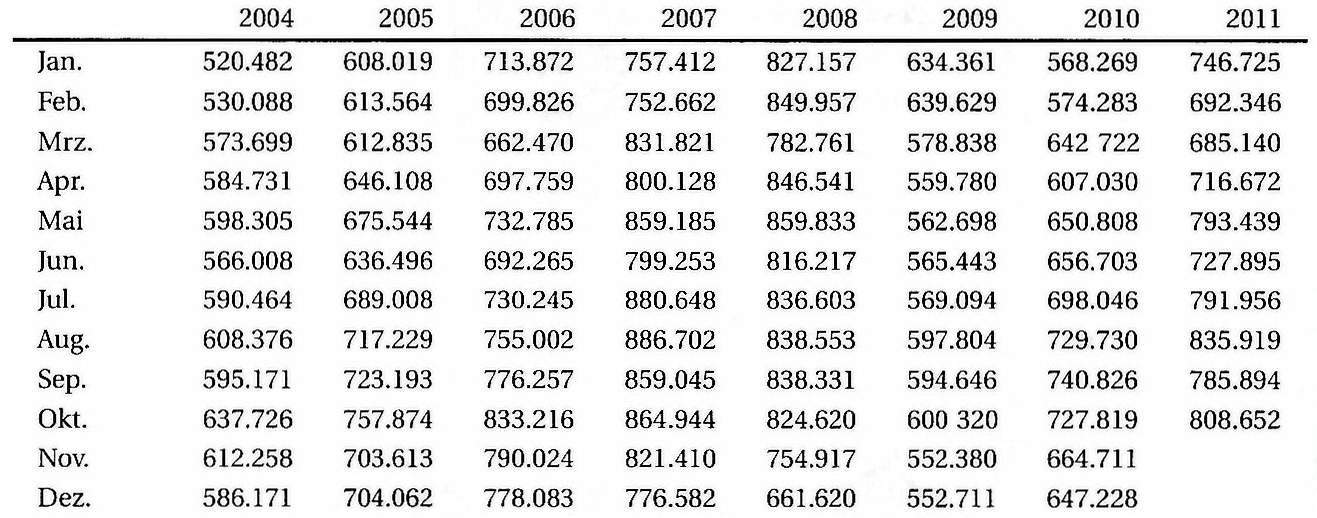
\includegraphics[width=1\textwidth]{Beispieldaten.png}
	\caption{Beispieldaten: Anzahl umgeschlagener Container\footnotemark}
	\label{tbl:Beispieldaten}
\end{table}
\footnotetext{\cite[S. 26.]{Wartala.2012}}

Die Information, welche mit MapReduce ermittelt werden soll, ist der Monat im Jahr 2004 mit den meisten umgeschlagenen Containern. Dieser Task lässt sich, unter Verwendung der erwähnten Unix-Tools, in drei Teilaufgaben separieren. Als erstes werden mit den \textit{grep}-Befehl alle Zeilen ausgegeben, welche aus dem Jahr 2004 stammen (siehe \autoref{lis:Grep2004}). Dieser Schritt repräsentiert den Mapper für dieses Beispiel. \\

\begin{lstlisting}[language=bash, caption=Befehl zur Anzeige aller Zeilen mit Jahr 2004, title=\autoref*{lis:Grep2004}: Befehl zur Anzeige aller Zeilen mit Jahr 2004\protect\footnotemark, label=lis:Grep2004]
grep 2004
\end{lstlisting}
\footnotetext{\cite[S. 27.]{Wartala.2012}}

Danach werden die Zeilen nach der dritten Spalte sortiert (Spalten wurden mit ; getrennt, siehe \autoref{lis:SortiereZeilen}). Dieser Befehl repräsentiert die Combine-Phase des Modells. \\

\begin{lstlisting}[language=bash, caption=Befehl zur Sortierung der Zeilen nach der dritten Spalte, title=\autoref*{lis:SortiereZeilen}: Befehl zur Sortierung der Zeilen nach der dritten Spalte\protect\footnotemark, label=lis:SortiereZeilen]
sort -t ';' -k +3 -r
\end{lstlisting}
\footnotetext{\cite[S. 27.]{Wartala.2012}}

Zuletzt wird die maximale Anzahl der Container bestimmt und das Jahr sowie der Monat und die Anzahl ausgegeben (siehe \autoref{lis:AusgabeBeispiel}). Dieser letzte Schritt in diesem Beispiel steht für den Reducer. \\

\begin{lstlisting}[language=bash, caption=Ausgabe des Beispielprogramms, title=\autoref*{lis:AusgabeBeispiel}: Ausgabe des Beispielprogramms\protect\footnotemark, label=lis:AusgabeBeispiel]
awk 'max== "" || $3 > max {max=$3;jahr=$1;monat=$2} END { print "jahr:" jahr; print "monat:" monat; print "anzahl:" max;}' FS=";"
\end{lstlisting}
\footnotetext{\cite[S. 27.]{Wartala.2012}}

Mit Hilfe der Unix-Befehls-Pipeline lassen sich alle Befehle auf eine Zieldatei Anwenden (siehe \autoref{lis:VollständigerBefehl}). Das Ergebnis wird in die Datei maximum\_umschlag.txt geschrieben.\footcite[Vgl.][S. 26 ff]{Wartala.2012} \\

\begin{lstlisting}[language=bash, caption=Vollständiger Befehl zur Auswertung der Beispieldaten, title=\autoref*{lis:VollständigerBefehl}: Vollständiger Befehl zur Auswertung der Beispieldaten\protect\footnotemark, label=lis:VollständigerBefehl]
cat container_umschlag.csv | grep 2004 | sort -t ';' -k +3 -r | awk 'max== "" || $3 > max {max=$3;jahr=$1;monat=$2} END { print "jahr:" jahr; print "monat:" monat; print "anzahl:" max;}' FS=";" | cat > maximum_umschlag.txt
\end{lstlisting}
\footnotetext{\cite[S. 28.]{Wartala.2012}}

Hier wird deutlich, dass es sich bei MapReduce nicht um einen Algorithmus, sondern um ein Vorgehensmodell handelt. Es geht lediglich darum, die Datenverarbeitung so effizient wie möglich sowohl parallel als auch seriell durchzuführen. Wie das Beispiel zeigt, lässt sich dieses Vorgehen auch sehr minimalistisch anwenden.

Für die Anwendung von MapReduce auf komplexere bzw. größere Daten reicht diese vereinfachte Form nicht mehr aus. Eine Lösung hierfür bietet das Hadoop Framework.

%<Noch ein paar sätze zur anwendung auf komplexere daten. Daraus die Überleitung zum nächsten Kapitel über Hadoop und das Framework schaffen>

%Woher kommt MapReduce? Wie funktioniert MapReduce? Stärken/Schwächen aufzeigen. Versuchen den Algorithmus mathematisch zu beschreiben ($O(n)$ Methode, Mengenleere). Hierfür muss noch Literatur gesucht werden. Bisher nur mathematische Beschreibungen im Internet gefunden.

%TODO: Einleitung ändern. Nicht direkt mit Zitat beginnen. Eher etwas in die richtung "Wartala sagt..." oder so
\section{Was ist Hadoop?}\label{sec:WasIstHadoop}
\flqq Kurz gesagt: Hadoop ist ein freies, Java-basiertes Open-Source-Framework für die skalierbare und verteilte Verarbeitung großer Datenmengen auf vielen Rechnern innerhalb eines Netzwerks.\frqq\footcite[S. 21]{Wartala.2012}

Die Entwicklung begann im Jahr 2004 durch den Programmierer Doug Cutting, nachdem dieser, im Rahmen des 6. Symposiums \ac{OSDI}, den Vortrag "`MapReduce - Simplified Data Processing on Large Clusters"', von den Google Mitarbeitern Jeffrey Dean und Sanjay Ghemawat, gehört hatte.

Zu diesem Zeitpunkt arbeitete Cutting an seinem Suchmaschinenprojekt mit dem Namen "`Nutch"', welches bereits 2002 ins leben gerufen wurde. Sein Ziel war eine leistungsfähige und konkurrenzfähige Softwarearchitektur, die es mit kommerziellen Suchmaschinen aufnehmen konnte. Bis 2004 konnte Nutch bereits 100 Mio. Webseiten mit nur vier Rechnerknoten indexieren.

Um jedoch das gesamte World Wide Web indexieren zu können, suchte Cutting gemeinsam mit der Nutch-Community nach einer Möglichkeit, die zugrundeliegende Architektur noch skalierbarer zu machen. Nach dem Vortrag bei der \ac{OSDI} fand Cutting eine passende Systemarchitektur in einem ebenfalls durch Dean und Ghemawat veröffentlichten Ansatz.\footcite[Näheres siehe][]{Dean.2004}

Gemeinsam mit zwei Teilzeit-Programmierern implementierte er ein, durch das Google Dateisystem \ac{GFS} inspiriertes, verteiltes Dateisystem, um darauf den MapReduce-Ansatz unter Nutch zu realisieren. 2006 wechselte Cutting zu Yahoo!. Das Dateisystem und MapReduce-Framework wurde aus Nutch extrahiert und in das eigenständige Apache-Projekt Hadoop überführt. Heute wird Hadoop in einer Reihe von Unternehmen produktiv eingesetzt, darunter Yahoo!, IBM und Microsoft.\footnote{Referenzzahlen für Unternehmen, die Hadoop einsetzen, unter:\\ \url{http://wiki.apache.org/hadoop/PoweredBy}}

Hadoop besteht aus zwei Kernkomponenten. Dem verteilten Dateisystem \ac{HDFS} und dem MapReduce-Framework. Dabei wird keine spezielle Servertechnik benötigt. Hadoop lässt sich sehr leicht auf Standardhardware betreiben.\footcite[Vgl.][S. 19-22]{Wartala.2012}

Die einzelnen Komponenten sind unabhängig voneinander einsetzbar. Eine große Rolle spielt bei Hadoop das Konzept der Datenlokalität. Entgegen dem normalen vorgehen, bei welchem einem Programm die Daten zu Verfügung gestellt werden, wird bei Hadoop das Programm zur Ausführung im Cluster verteilt. Da es sich bei Hadoop i.d.R. um Anwendungen im Big Data Bereich handelt, macht es Sinn, da die Anwendung wesentlich kleiner und somit schneller zu übertragen ist, als die Daten.\footcite[Vgl.][S. 20]{Freiknecht.2014}

\subsection{Das verteilte Dateisystem HDFS}\label{subsec:DasVerteilteDateisystemHDFS}
Den Kern, und somit die wichtigste Funktion von Hadoop, Bilder das Dateisystem. Aktuell werden Daten zum Großteil in relationalen Datenbanken gespeichert. Parallel existiert noch die Möglichkeit, Daten ohne Relation direkt auf einem herkömmlichen Dateisystem abzulegen (sog. Flat-Files). Da die Verteilung und Verwaltung großer Datenmengen in einem Cluster sehr aufwändig ist, wurde, angelehnt an das \ac{GFS}, \ac{HDFS} entwickelt. Dabei wurden die folgenden Anforderungen an das Design des Dateisystems gestellt:

\begin{itemize}
	\item Betrieb auf \gls{Commodity-Hardware}
	\item Ausfallsicherheit einzelner Knoten
	\item Speicherung und Verarbeitung großer Datenmengen
	\item Einfache Skalierbarkeit\footcite[Vgl.][S. 21]{Freiknecht.2014}
\end{itemize}

Dabei macht sich \ac{HDFS} zusätzlich die bekannten Eigenschaften verteilter Dateisysteme zunutze. Der \textit{Parallelisierung}, dem gleichzeitigen Lesen und Schreiben von Dateien, verteilt im Netz auf vielen Rechnern. Der \textit{Cluster-lokalen Verarbeitung}, bei der die Verarbeitungsprozesse auf den Knoten im Cluster ausgeführt werden, welche die Daten halten, um die Kommunikation im Netzwerk so gering wie möglich zu halten. Zuletzt dem \textit{Failover}-Prinzip, bei dem die Daten auf die einzelnen Knoten blockweise und gleichmäßig verteilt werden.

Mittels \ac{HDFS} ist Hadoop in der lage, große Datenmengen auf kostengünstiger Standarthardware zu speichern, im Vergleich zu kostspieligen Speichernetzwerken (\ac{SAN} oder \ac{NAS}). 

Die Architektur von \ac{HDFS} entspricht einem Master-Slave-System. Die verschiedenen Aufgaben verteilen sich auf zewi unterschiedliche Dienste. Dem NameNode (Master) und den DataNodes (Slaves). \autoref{fig:HDFSArchitekturSchema} zeigt das Architektur-Schema. Innerhalb einer Hadoop-Infrastruktur gibt es immer nur einen NameNode, welcher $n$ DataNodes ansteuert.

Die genaue Funktionsweise von \ac{HDFS} wird in einem Comic\footnote{Comic über Funktionsweise von HDFS: \\ \url{http://de.slideshare.net/jaganadhg/hdfs-10509123}} von \textit{Maneesh Varshney} sehr einfach und anschaulich erklärt.\footcite[Vgl.][S. 22 f.]{Wartala.2012}

\begin{figure}[h]
	\centering
	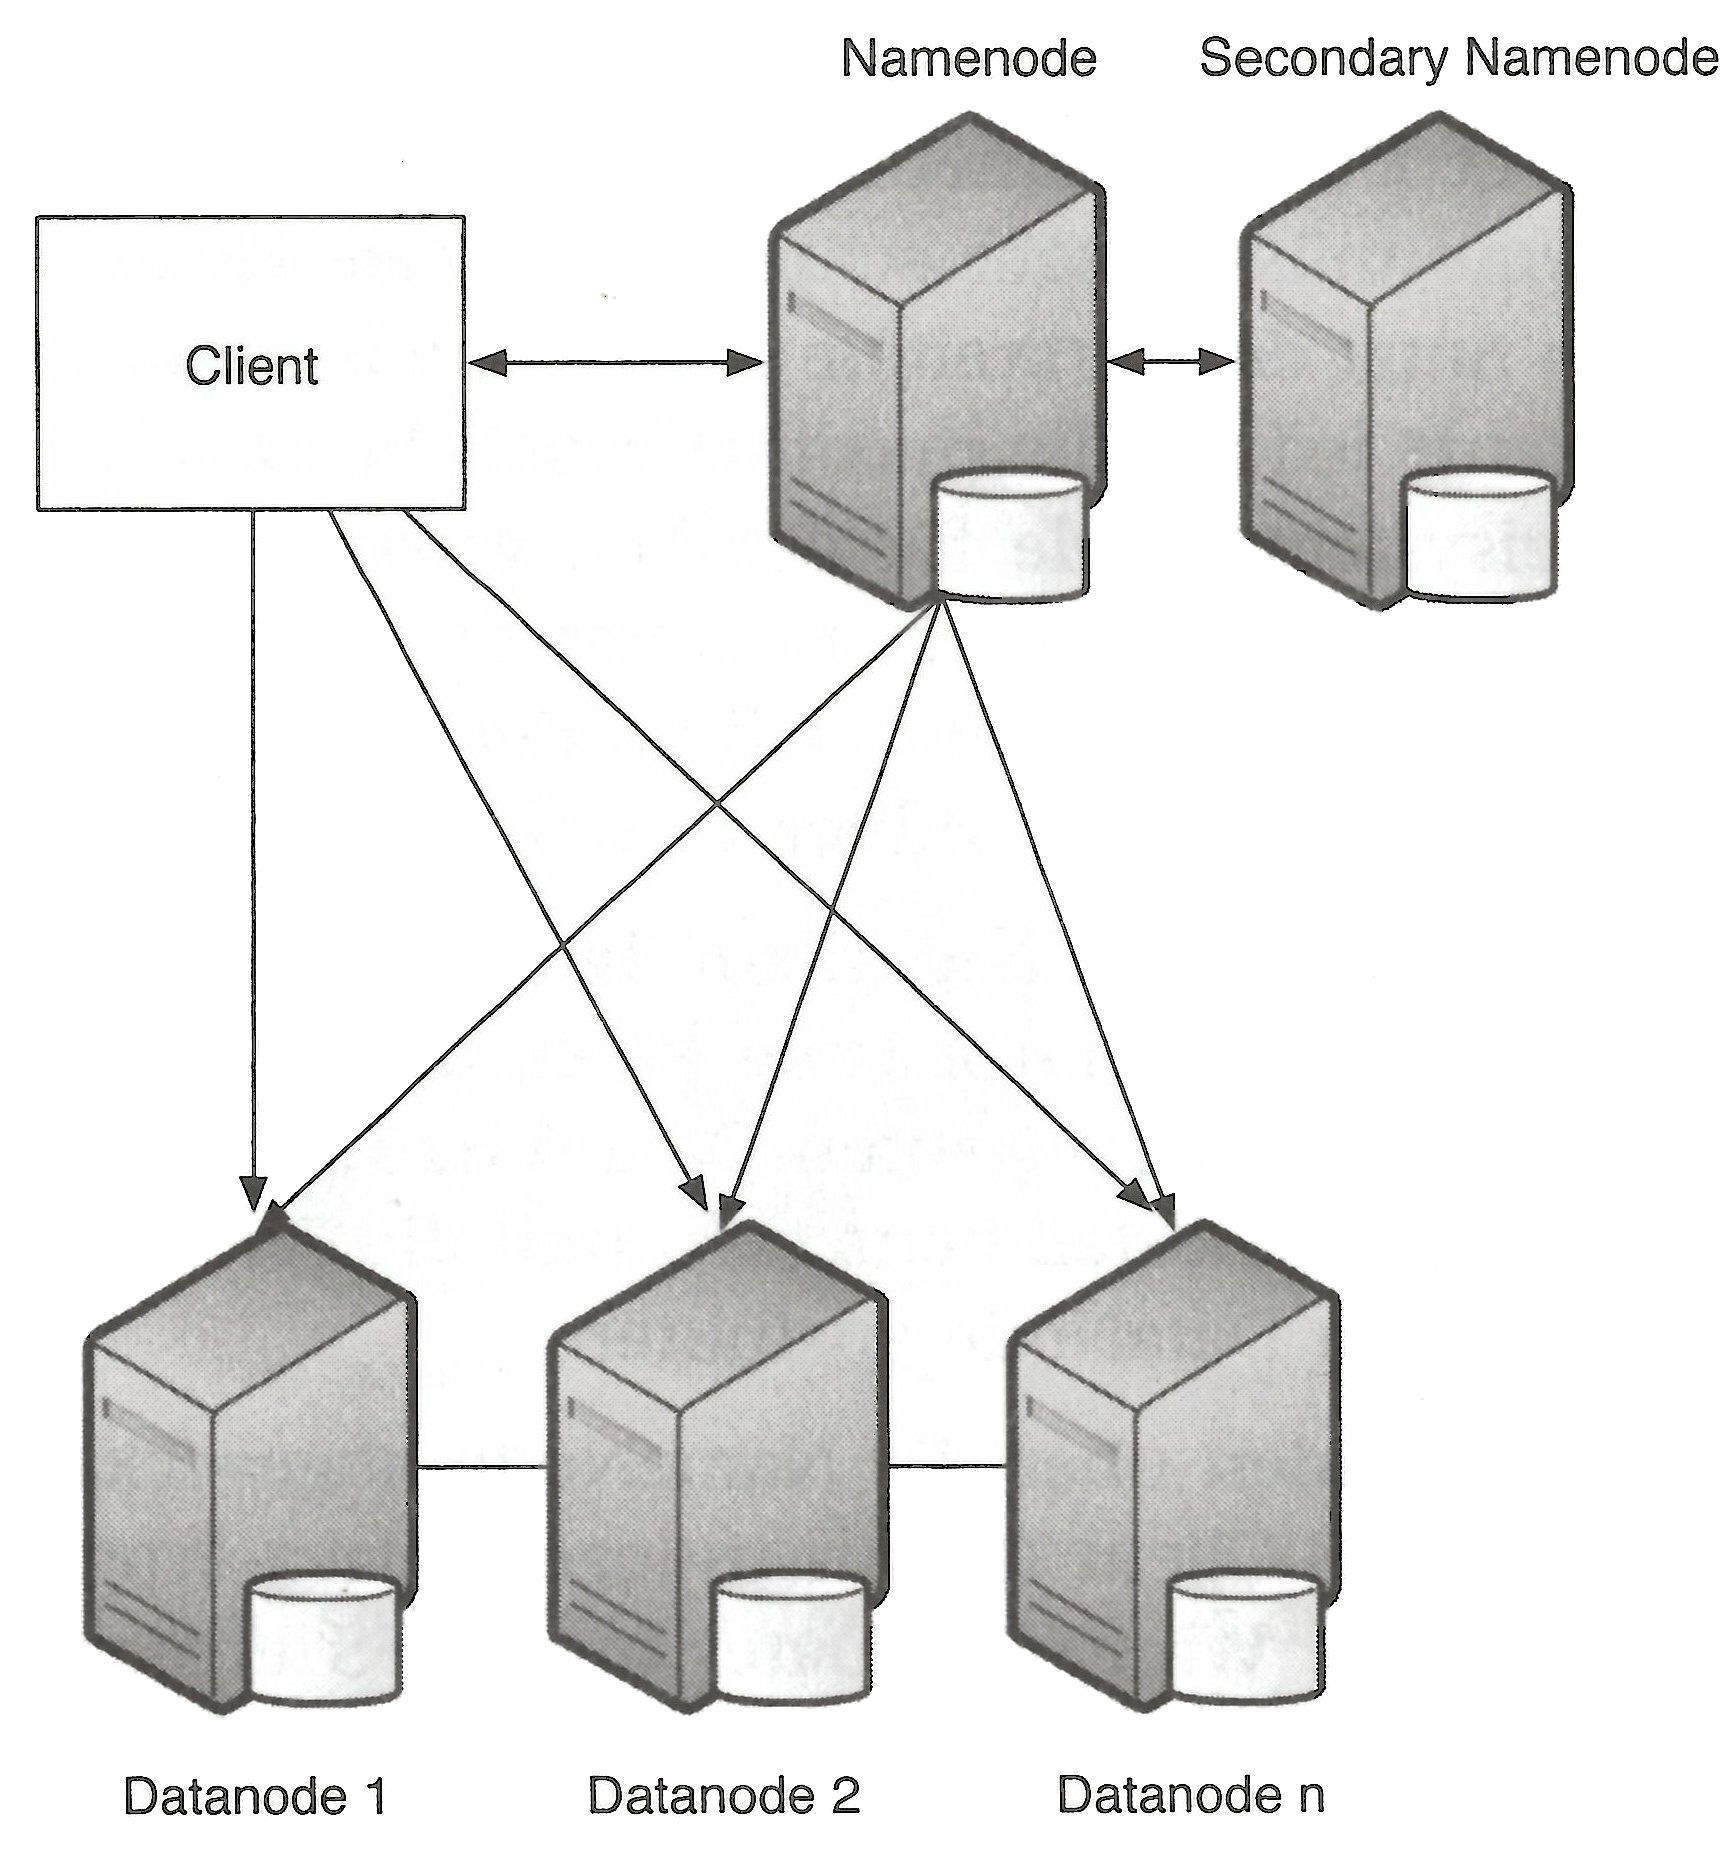
\includegraphics[scale=1.2]{HDFS_Architektur.png}
	\caption{HDFS Architektur-Schema\footnotemark}
	\label{fig:HDFSArchitekturSchema}
\end{figure}
\footnotetext{\cite[S. 23.]{Wartala.2012}}

\subsubsection{NameNodes}
Der NameNode kontrolliert und regelt alle Dateioperationen, welche auf das Dateisystem ausgeübt werden sollen. Er stellt den Master des Systems dar, und kümmert sich um die Speicherung der Dateinamen, Verzeichnisse und Zugriffe. Dabei koordiniert er die Verteilung der Dateiblöcke im Cluster und überwacht die ihm bekannten Slave Knoten (DataNodes). Der NameNode speichert lediglich Metainformationen über die im Dateisystem gespeicherten Daten. Die Daten selbst werden von ihm an die DataNodes weiter geleitet. Zusammengefasst sind die Aufgaben des NameNode:

\begin{itemize}
	\item Speicherung der Metadaten im Hauptspeicher
	\item Verteilung der Datenblöcke
	\item Überwachung der DataNodes, um Ausfälle oder beschädigte Daten schnell erkennen zu können.
\end{itemize}

Da alle Metadaten des Dateisystems im Hauptspeicher des NameNodes gehalten werden, ist die Anzahl der Dateien, die im \ac{HDFS} abgelegt werden können, begrenzt. Die Datenblöcke sind i.d.R. zwischen 64 und 128 \ac{MB} groß (im Gegensatz zu traditionellen Dateisystemen, welche mit Blöcken in der Größe 1 bis 64 \ac{KB}). Für die Verwaltung eines einzelnen Datenblocks benötigt der NameNode ca. 150 Byte. Bei einer Hauptspeichergröße von 1 \ac{GB} können i.d.R. mehr als 6 Mio. Dateien und Ordner verwaltet werden.\footcite[Vgl.][S. 24]{Wartala.2012}

Alle Anfragen an das \ac{HDFS} laufen über den NameNode. Dabei werden die Befehle von einem \ac{HDFS}-Client gesendet (Kommandozeile, Java-Programm, etc.). Die im Zuge der Bachelorarbeit programmierte Anwendung verwendet das Java \ac{API}, welches von Hadoop bereitgestellt wird.

\subsubsection{DataNodes}
DataNodes sind die Slave Knoten des Dateisystems, in welchen die Datenblöcke gespeichert werden. Sie besitzen keine Informationen über die Daten selbst. Aufgaben der DataNodes sind:

\begin{itemize}
	\item Verwaltung der einzelnen Dateisystem-Blöcke
	\item Dateisystem innerhalb einer Replikationskette (Replication chain)
	\item Zustandsinformationen (über sich selbst und die Daten) für NameNode bereitstellen
\end{itemize}

Zudem werden die MapReduce-Prozesse auf genau den Knoten ausgeführt, welche die benötigten Daten besitzen. DataNodes replizieren selbstständig die durch den NameNode übermittelten Daten an weitere DataNodes, wenn ihnen Dies durch den Master mitgeteilt wird. Zudem können sie, nach einer entsprechenden Anweisung des NameNodes, beschädigte Datenblöcke von anderen DataNodes kopieren und ersetzen.\footcite[Vgl.][S. 25 f.]{Wartala.2012}

%<Was ist ein verteiltes Dateisystem überhaupt und wozu braucht man es? Vergleich mit einem normalen Dateisystem?>

%\subsection{MapReduce-Framework}\label{subsec:MapReduceFramework}
%ACHTUNG. Vermutlich überflüssig da MapReduce bereits beschrieben wurde. Das Framework funktioniert nicht wirklich anders es stellt nur interfaces bereit damit die klassen stimmen.

\subsection{Abgrenzung - Was ist Hadoop nicht?}
Es gibt unterschiedliche Techniken für die Speicherung und Verarbeitung von Daten, mit ihren jeweiligen Stärken und Schwächen. Es gibt eine Reihe von Kritikern, welche dem MapReduce-Ansatz unterschiedlichste Mängel vorwerfen. Darunter u.a. das der Ansatz nicht wirklich innovativ und würde Funktionen wie Loadbalancing, Transaktionen oder auch Views vermissen.

Es ist daher wichtig zu wissen, was Hadoop nicht ist. Jede Technologie ist nur dann Sinnvoll, wenn sie der Aufgabe entsprechend eingesetzt wird. Für die Aufgaben, für welche Hadoop konzipierte wurde, sind keine Transaktionen oder Views notwendig. Diese Funktionalitäten werden bei relationalen Datenbanken (und deren Aufgaben) benötigt, nicht jedoch bei Hadoop.

%TODO: Abwägen ob dieser Absatz in das Kapitel "Was ist Hadoop" gehört. Meine Idee war, dass dieser Absatz die Abgrenzung zu relationalen Datenbanksystemen verdeutlichen sollte.
Laut Wartala gibt es eine Reihe von algorithmischen Problemlösungen, welche i.d.R. auf Hadoop besser ausgeführt werden können, als auf einem relationalen Datenbanksystem. Darunter unter anderem die Indexierung für Suchmaschinen, Text Mining, sowie die Analyse von Logfiles und Click-Streams.

Eine weitere Unterscheidung muss zu Systemen gemacht werden, welche in die Gruppe der \ac{EDA} bzw. \ac{CEP} Systeme fallen. Der Fokus von Hadoop liegt bei der Verarbeitung großer Datenmengen mittels Batch-Prozessen. Dieser Ansatz ist zu langsam für eine Real- oder Near-Time-Datenverarbeitung. Jedoch ist das Ziel eines \ac{EDA} oder \ac{CEP} Systems nicht die Abfrage gespeicherter Informationen, sondern die kontinuierliche Informationsbeschaffung, und haben somit eine vollkommen andere Funktion.

Eine letzte Abgrenzung muss zum sog. Grit Computing erfolgen. Hadoop konzentriert sich auf die Transformation von Schlüssel-Wert-Paaren innerhalb der MapReduce-Funktionen, und kann auf einer großen Zahl identischer Hardware installiert und ausfallsicher betrieben werden. Grid-Systeme dagegen verteilen Daten und Algorithmen auf einem niedrigeren Abstraktionsniveau. Dabei können einzelne Prozesse, über die im Grid Computing bekannte Schnittstelle \ac{MPI}, innerhalb eines Netzwerkes komplexere Nachrichten und Objekte austauschen. Grid-Systeme können somit mehr als nur Schlüssel-Wert-Paare verteilen. Eine solche komplexität ist bei Hadoop jedoch nicht notwendig.\footcite[Vgl.][S. 30-33]{Wartala.2012}

Das Fehlen dieser Funktionen zu kritisieren ist daher nicht sinnvoll. Es ist die Kombination unterschiedlicher Technologien, für ihren jeweiligen erdachten Zweck, die eine Architektur erfolgreich macht. \flqq Nicht ohne Grund betreibt der Erfinder des MapReduce-, \ac{GFS}- und BigTable-Ansatzes, Google, die weltgrößte MySQL-Installation.\frqq\footcite[S. 31]{Wartala.2012}

%<Was gehört alles zu Hadoop? Worauf zieht Hadoop ab? Warum verwende ich Hadoop statt es einfach selbst zu machen? Stärken und Schwächen aufzeigen.>

\subsection{Überlegungen zur Ausfallsicherheit von Hadoop}
Sowohl Wartala als auch Freiknecht, schreiben in ihren Büchern über die Ausfallsicherheit von Hadoop. Durch die Replikation eines Datenblocks auf unterschiedliche DataNodes, stehen die Daten selbst bei einem Ausfall eines Knotens zu Verfügung. Das Dateisystem kann so konfiguriert werden, dass es nicht nur über die Anzahl der DataNodes Kenntnis besitzt, sondern ebenfalls über deren Standort (anderer Server, Rack oder anderes Rechenzentrum).

In einer komplexeren Infrastruktur, mit mehreren DataNodes, verteilt auf unterschiedliche Racks, folgt Hadoop zwei grundsätzlichen Regeln bei der Replikation von Datenblöcken:

\begin{enumerate}
	\item Nur eine Replikation pro DataNode
	\item Nur maximal zwei Replikationen im gleichen Rack
\end{enumerate}

Die Knoten melden sich in regelmäßigen Abständen beim NameNode, um, zum einen, mitzuteilen dass sie noch aktiv sind, und um einen Abgleich der Datenblöcke mittels einer Checksumme vor zu nehmen. Sollte diese nicht stimmen, kann der NameNode dem betreffenden DataNode den Auftrag erteilen, den Datenblock von einem anderen Knoten zu kopieren. Dadurch wird der beschädigte Block ersetzt. Die Integrität der Daten ist somit durch die Replikation sehr sicher.

Es gibt jedoch einen großen Schwachstelle in Form des im System einmalig vorhandenen NameNodes. Dieser stellt einen \ac{SPOF} dar. Ein Ausfall des NameNode würde das gesamte Dateisystem lahm legen. Zudem besteht die Gefahr, dass, bei einem plötzlichen Ausfall des NameNode, die gespeicherten Metadaten beschädigt oder verloren gehen.

Aus diesem Grund muss der NameNode über entsprechende Sicherheitsvorkehrungen verfügen, um das Ausfallrisiko zu minimieren.

%<Verteilung der Replikationen über mehrere DataNodes in verschiedenen Racks, Single Point of Failor!>

%\section{Betrachten von Alternativen}
%Alternativen sowohl zu Hadoop als auch zu MapReduce selbst. Was gibt es in diesen Bereichen noch? Wie unterscheiden sich diese?
%TODO: Alternativen in 3.3 und 5.1 oder eher 5.4 betrachten/erwähnen
